\documentclass[russian, utf8, nocolumnxxxi, nocolumnxxxii, 14pt]{eskdtext}
\usepackage[utf8]{inputenc}
\usepackage[T1,T2A]{fontenc}
\usepackage[english, russian]{babel}
\usepackage[argument]{graphicx}
\usepackage{graphicx}
\graphicspath{{images/}}
\usepackage{wrapfig}
\usepackage{tikz}
\usepackage{siunitx}
\usepackage[american,cuteinductors,smartlabels]{circuitikz}
\setlength{\parskip}{0pt}
\renewcommand{\baselinestretch}{1.25}
\renewcommand{\ESKDtheTitleFieldX}{2018}

\ESKDdepartment{МИНОБРНАУКИ РОССИИ}
\ESKDcompany{
САНКТ-ПЕТЕРБУРГСКИЙ ГОСУДАРСТВЕННЫЙ \\
ЭЛЕКТРОТЕХНИЧЕСКИЙ УНИВЕРСИТЕТ\\
«ЛЭТИ» ИМ. В.И. УЛЬЯНОВА (ЛЕНИНА)\\
Кафедра робототехники и автоматизации\\ 
производственных систем}
\ESKDtitle{ПОЯСНИТЕЛЬНАЯ ЗАПИСКА К КУРСОВОЙ РАБОТЕ}
\ESKDdocName{по дисциплине "Информатика"\\
Тема: Решение математических задач с использование математических пакетов Scilab и Reduce-algebra\\
Вариант 22}
\ESKDtitleDesignedBy{Студент группы 8871}{Турыгин Д.А.}
\ESKDtitleDesignedBy{Старший преподаватель}{Прокшин А.Н.}
\ESKDauthor{Турыгин}
\ESKDchecker{Прокшин}
\ESKDcolumnI{\small Решение математических задач с использование математических пакетов Scilab и Reduce-algebra}
\ESKDcolumnIX{СПбГЭТУ гр.8871}

\begin{document}
\maketitle
\newpage
Содержание\\
\indent 1. Постановка задачи курсовой работы.\\
\indent 2. Задание для выполнения курсовой работы.\\
\indent 3. Функции.\\
\indent 3.1 Решение уравнения.\\
\indent 3.2 Исследование функции.\\
\indent 4.\\
\indent 4.\\
\indent 4.\\

\newpage
\section{Постановка задачи курсовой работы.} \\
\indent Цель курсовой работы: уметь применять персональный компьютер и
математические пакеты прикладных программ в инженерной деятельности.\\
\indent Тема курсовой работы: решение математических задач с использованием математического пакета "Scilab" или "Reduce-algebra".
\newpage
\section{Задание для выполнения курсовой работы.}\\
1. Даны функции $f(x) = \sqrt{3}sin(x) + cos(x)$ и $g(x) = cos(2x + \pi/3) - 1$ \\
\indent а) Решить уравнение $f(x) = g(x)$. \\
\indent б) Исследовать функцию  $h(x) = f(x) - g(x)$ на промежутке $[0;\frac{5}{6}\pi]$\\
\indent 2. Найти коэффициенты кубического сплайна, интерполирующего данные, представленные в векторах $V_x$ и $V_y$.\\
Построить на графике функцию $f(x)$, полученную после нахождения коэффициентов кубического сплайна.\\
\indent Представить графическое изображение результатов интерполяции исходных данных различными методами с использованием встроенных функций splin(x, y, "natural"), splin(x, y, "clamped"), splin(x, y, "not$_$a$_$knot"), splin(x, y, "fast"), splin(x, y, "monotone") и interp(xx, x, y, d).\\
\indent 3. Решить задачу оптимального распределения неоднородных ресурсов. На предприятии постоянно возникают задачи определения оптимального плана производства продукции при наличии конкретных ресурсов (сырья, полуфабрикатов, оборудования, финансов, рабочей силы и др.) или проблемы оптимизации распределения неоднородных ресурсов на производстве.\\
\indent Пусть в распоряжении завода железобетонных (рисунок 1) изделий имеется m видов сырья в объемах $a_i$. Требуется произвести продукцию $n$ видов. Дана технологическая норма $ci_j$ потребления отдельного $i$-го вида сырья для изготовления единицы продукции каждого $j$-гo вида. Известна прибыль $\Pi_j$, получаемая от выпуска единицы продукции $j$-гo вида. Требуется определить, какую продукцию и в каком количестве должен производить завод, чтобы получить максимальную прибыль.\\
\begin{center} 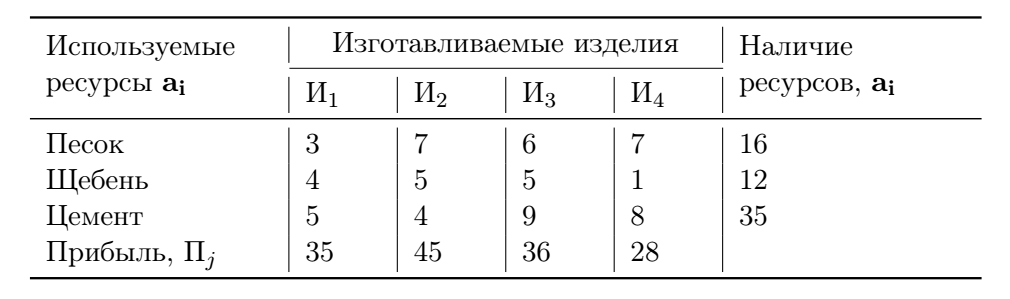
\includegraphics[scale=0.4]{JPG/ein.png}\\
Рисунок 1 -- Количество ресурсов находящихся в расворяжении завода.\\
\end{center}
\newpage
\section{Функции}
\subsection{Решение уравнения}
Даны функции $f(x) = \sqrt{3}sin(x) + cos(x)$ и $g(x) = cos(2x + \pi/3) - 1$ \\
\indent Задача решения уравнения $f(x) = g(x)$ эквивалентна нахождению корней уравнения $h(x) = f(x) - g(x)$:\\
\begin{center} $y = \sqrt{3}sin(x) + cos(x) - cos(2x + pi/3) + 1$ \end{center}\\
\indent Для того чтобы понять характер данного уравнения, построим график его функции (рисунок 2):\\
$function y = h(x)$ \\
$y = sqrt(3) * sin(x) + cos(x) - cos(2*x + \%pi/3) + 1$ \\
$endfunction$ \\
$plot(0:0.01:2*\%pi,h)$ \\
\begin{center} 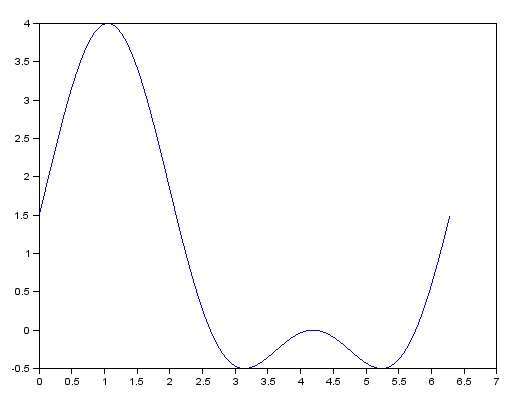
\includegraphics[scale=0.9]{JPG/zwei.jpg}\\
Рисунок 2 -- График функции\\
\end{center}
\indent Исходя из вида данного графика, можно сказать, что уравнение имеет от 2-ух до 4-ёх корней. Для получения данных корней применим функцию $fsolve$ задав вектор начальныч приближеных значений решения уравнения $x0$ (на основе построенного графика в точках $x0_1$ = 3, $x0_2$ = 4.2, $x0_3$ = 4.3, $x0_4$ = 5.5) получим вектор решений заданного уравнения $x$. $v$ -- вектор значений функции в точках $x$. \\
\indent Находим корни уравнения: \\
$deff('y=h(x)','y=sqrt(3)*sin(x)+cos(x)-cos(2*x+\%pi/3)+1')$ \\
$x0=[3,4.2,4.3,5.5]$; \\
$[x,v]=fsolve(x0,h)$ \\
 $v$  = \\
-2.220D-16 \quad 0. \quad 0. \quad 7.772D-16 \\
 $x$  = \\
   2.6179939 \quad 4.1887902 \quad 4.1887902 \quad 5.759586 \\
\indent Уранение имеет 3 корня: $x_1$ = 2.6179939, $x_2$ = 4.1887902 и $x_3$ = 5.759586. 
\indent Вследствие того, что решенное уравнение является тригонометрическим, можно предположить о кратности полученных решений числу $\pi$:\\
$x/\%pi$\\
 ans  =\\
   0.8333333 \quad 1.3333333 \quad 1.3333333 \quad 1.8333333\\
\indent Домножим данные решения на 3:\\
$3*x/\%pi$ \\
 ans  = \\
   2.5 \quad 4. \quad 4. \quad 5.5\\
\indent Полученые корни запишем в тригонометрической форме:\\
\begin{center}
$x_1 = \frac{5}{6}\pi + 2n\pi, n \in Z$\\
$x_2 = \frac{8}{6}\pi + 2n\pi, n \in Z$\\
$x_3 = \frac{11}{6}\pi + 2n\pi, n \in Z$\\
\end{center}
\subsection{Исследование функции.}

\end{document}
